\section{Unique Approaches}

To apply perceptron Q-learning to Super Smash Brothers Melee, we apply unique techniques to deal with discontinuities in optimal behavior, state-evolution, and delays between an action and its result.

\subsection{Discontinuity in Optimal Behavior}
In Super Smash Brothers Melee, the optimal action largely depends on the current state. An issue arises in global-approximation techniques when nearby states should have dissimilar optimal actions. An example of this is the case of an agent standing on the edge of the stage, in which its goal is to deal damage to the opponent, and an agent being slightly off of the stage (about to fall to its death unless some preventative action is taken), in which it should make an effort to navigate back to the stage and avoid dying. 

To prevent generalization from nearby but dissimilar states, we discretize the environment into an additional three super-states: off the stage to the left, on the stage, and off the stage to the right. These super-states represent different situations in which the optimal behavior of the agent should be unique from a nearby position that is in a different super-state. As discussed in the applications section, the padded beta vector results in differently trained perceptron weights in different super-states for each map partition. This improves the agents ability to survive after being knocked off of the stage because the agent learns to jump back towards the stage in an effort to survive (and avoid penalties for dying). 


\subsection{State Evolution}
Another issue we address was the impact of ”action-lockout”, in which an action taken may have no impact on the agents transition to the next state. An example of this is when the agent selects an action with a long wind-up animation that cannot be canceled by inputting other actions. To address this, actions that are taken during an "action-lockout" are ignored during the training process of the basis function weights. 

While performing batch learning, this is taken into account. In the weight update process, $\theta_a\beta(s)$ of the last action take is used for each update, while the state $s'$ is taken as usual. The rewards are computed at each state step and assigned back to the last action taken. The result is that the original state action pair is rewarded for the state evolution that occurs, rather than rewarding the action at intermediate states of the evolution. 

\begin{figure}[!htb]
	\centering
	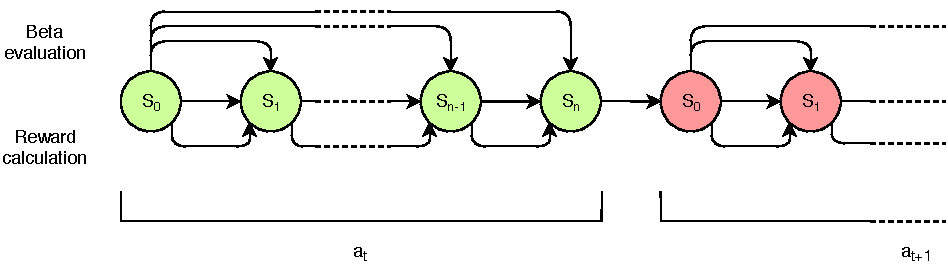
\includegraphics[width=120mm]{stateevolution.pdf}
	\caption{State evolution diagram}
	\label{fig:stateevo}
\end{figure}

Figure~\ref{fig:stateevo} is a representation a state evolution. All the green states indicate a single state evolution with action-lockout occurring at each new state $S_{t}$. The transition to the red states are when an action is taken that affect the transition to the next state, starting a new state evolution. We can see the how the reward is calculated from $S_{t}$ to $S_{t+1}$ while the beta function is evaluated from $S_{0}$ to $S_{t+1}$.

\subsection{Action Impact Delay}

Dealing with rewards for kills and deaths is not straight forward due to a large time delay between an action that results in one of these events and the event occurring. To assign rewards to killing the opponent, the last action the agent take that deals damage is recorded as a "last damaging action". When the opponent dies, a large reward is assigned to this "last damaging action". This is necessary to avoid assigning large rewards to actions that do not cause the opponent to die, and is equivalent to knowing immediately after the action is taken if it will result in the death of the opponent.





